\chapter{Dualité de Fourier, quantité de mouvement et mouvement d’une particule libre}

\section{Des fondements aux exemples}

L’intrication est au cœur de la mécanique quantique, mais ses fondements sont maintenant suffisamment exposés pour que nous puissions commencer à les utiliser. Jusqu’ici, le cours s’est appuyé sur des systèmes volontairement simples : un spin, un appareil orientable, un nombre fini de résultats possibles et des mesures répétées permettant d’inférer des probabilités. Ces expériences sont logiquement plus simples que le chemin historique qui a conduit à la découverte de la mécanique quantique, mais elles en contiennent les ingrédients opérationnels minimaux.

\begin{classroomqa}
\audiencequestion{Quel rôle jouent, en mécanique quantique, les quelques points de départ empiriques de Newton ?}
\lecturerresponse{Un modèle minimal est l’appareil de mesure de spin orientable. On prépare un spin, on choisit un axe, on actionne la commande de mesure, on note \(+1\) ou \(-1\), puis on répète l’expérience jusqu’à connaître les fréquences des résultats. L’espace vectoriel, les observables, les amplitudes et la règle de Born organisent ces statistiques. Historiquement, la théorie est née d’un ensemble bien plus riche de phénomènes atomiques, mais cette expérience à deux résultats suffit, sur le plan logique, à en faire apparaître la structure.}
\end{classroomqa}

\begin{classroomqa}
\audiencequestion{Faut-il répéter la même procédure statistique pour chaque grandeur physique, par exemple le spin ou la quantité de mouvement ?}
\lecturerresponse{Oui. Une observable est associée à une classe de dispositifs expérimentaux et de résultats possibles. Le formalisme prédit la distribution une fois spécifiés l’état et l’observable, mais le sens physique de l’observable est ancré dans la manière dont on la mesure.}
\end{classroomqa}

Avant de quitter l’intrication, répondons complètement à une question soulevée dans la discussion précédente. Considérons deux électrons avec des secteurs singulet et triplet, et ajoutons le champ de rayonnement comme autre sous-système quantique. Le champ de rayonnement possède un état de vide \(\ket{0_\gamma}\) et un état à un photon \(\ket{1_\gamma}\). Le nombre de particules lui-même peut être en superposition ; rien ne restreint la superposition à différents états d’un nombre de particules fixé.

Pour la transition idéalisée discutée en cours, un état initial des électrons non intriqué peut s’écrire comme une superposition de composantes singulet et triplet,
\begin{equation}
\ket{\uparrow\downarrow}
=
\frac{1}{\sqrt{2}}
\left(\ket{S}+\ket{T_0}\right).
\end{equation}
En l’absence de photon initial, l’état est
\begin{equation}
\ket{\Psi(0)}
=
\frac{1}{\sqrt{2}}
\left(\ket{S}+\ket{T_0}\right)
\otimes\ket{0_\gamma}.
\label{eq:l9-initial-radiative-state}
\end{equation}
La composante singulet reste un singulet sans émission, tandis que la composante triplet excitée peut se désexciter vers le singulet en émettant un photon :
\begin{align}
\ket{S}\ket{0_\gamma}
&\longrightarrow
\ket{S}\ket{0_\gamma}, \\
\ket{T_0}\ket{0_\gamma}
&\longrightarrow
\ket{S}\ket{1_\gamma}.
\end{align}
La linéarité donne alors
\begin{equation}
\ket{\Psi_{\mathrm{final}}}
=
\ket{S}\otimes
\frac{\ket{0_\gamma}+\ket{1_\gamma}}{\sqrt{2}}.
\label{eq:l9-final-radiative-state}
\end{equation}

\begin{figure}[htbp]
\centering
\includegraphics[width=0.88\textwidth]{lecture_09_figure_01.png}
\caption{Avant la relaxation radiative, l’état des électrons est décomposé en composantes singulet et triplet, puis tensorisé avec le vide photonique.}
\lectureframe{00:05:10}
\end{figure}

L’expression finale est un produit tensoriel entre la paire d’électrons et le champ de rayonnement. Les deux électrons sont intriqués l’un avec l’autre, car \(\ket{S}\) est intriqué, tandis que le champ de rayonnement se trouve dans une superposition de zéro et d’un photon. Cet exemple est subtil, car l’interaction a redistribué l’intrication : l’état initial en produit des électrons évolue vers une paire d’électrons intriqués, alors que l’état final idéalisé des électrons et du rayonnement se factorise.

\begin{classroomqa}
\audiencequestion{Un photon incident quelconque pourrait-il inverser la transition et désintriqu­er les électrons ?}
\lecturerresponse{Non. Le processus renversé dans le temps exige l’état photonique, le mode, la phase, l’énergie et l’historique d’interaction appropriés. Renvoyer le photon émis était une façon abrégée de décrire la mise en place de l’évolution inverse du système fermé tout entier ; cela ne signifie pas qu’un photon quelconque annulerait l’intrication.}
\end{classroomqa}

\begin{classroomqa}
\audiencequestion{Qu’est-ce qui fait émettre un photon au triplet si aucun champ magnétique extérieur n’a été introduit ?}
\lecturerresponse{Les électrons interagissent entre eux et avec le champ électromagnétique quantifié. Leur interaction dépendant du spin rend énergétiquement favorable l’une des configurations de spin, et l’excès d’énergie peut être évacué sous forme de rayonnement. Aucun appareil de mesure externe n’est nécessaire : il s’agit de la dynamique unitaire ordinaire du système composé des électrons et du champ.}
\end{classroomqa}

Ce point réglé, oublions maintenant le spin et étudions le problème de mouvement le plus simple : une particule sur une droite à une dimension.

\section{Ondes planes et paire de Fourier}

Avant de revenir à la physique, il nous faut une parenthèse mathématique. Commençons par
\begin{equation}
e^{ipx}=\cos(px)+i\sin(px).
\end{equation}
À ce stade, \(p\) est simplement un nombre réel qui règle la fréquence d’oscillation. L’expression ne dépend pas du temps et ne décrit donc pas encore une onde en mouvement. On l’appelle onde plane parce que, en fonction de \(x\), elle a la forme sinusoïdale familière.

Une vaste classe de fonctions suffisamment régulières peut être décomposée en de tels modes. Nous nous limitons aux fonctions qui se comportent assez bien pour que les intégrales ci-dessous soient définies : elles ne doivent pas diverger à l’infini spatial, et les fonctions d’onde physiques que nous étudierons par la suite seront de carré intégrable. Avec une convention de normalisation symétrique, la paire de Fourier s’écrit
\begin{align}
\psi(x)
&=
\int_{-\infty}^{\infty}
\frac{dp}{\sqrt{2\pi}}\,
\widetilde{\psi}(p)e^{ipx},
\label{eq:l9-fourier-forward}\\
\widetilde{\psi}(p)
&=
\int_{-\infty}^{\infty}
\frac{dx}{\sqrt{2\pi}}\,
\psi(x)e^{-ipx}.
\label{eq:l9-fourier-inverse}
\end{align}
Le coefficient \(\widetilde{\psi}(p)\) est l’amplitude complexe du mode d’étiquette de Fourier \(p\). Les facteurs \(1/\sqrt{2\pi}\) sont conventionnels ; en plaçant l’un dans chaque sens, les deux formules prennent une forme réciproque. Le signe relatif moins dans l’exposant est essentiel.

\begin{figure}[htbp]
\centering
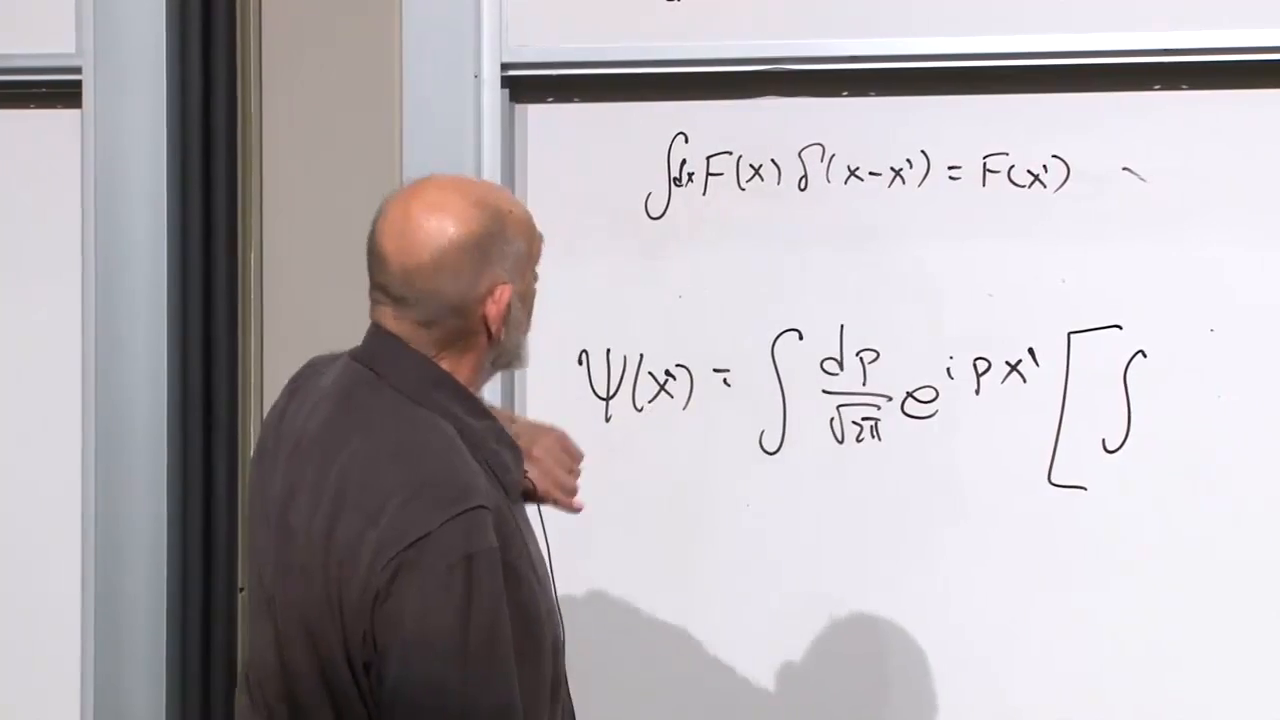
\includegraphics[width=0.88\textwidth]{lecture_09_figure_02.png}
\caption{La paire de Fourier symétrique : une fonction est décomposée en ondes planes, et les amplitudes des modes sont obtenues par la transformée inverse.}
\lectureframe{00:14:35}
\end{figure}

\begin{classroomqa}
\audiencequestion{\(\psi(x)\) et \(\widetilde{\psi}(p)\) sont-elles censées être complexes ?}
\lecturerresponse{En général, oui. Une fonction particulière peut être réelle, auquel cas ses coefficients de Fourier satisfont une relation de conjugaison supplémentaire. Mais les amplitudes quantiques sont naturellement complexes, et nous n’imposons ici aucune condition de réalité.}
\end{classroomqa}

\begin{classroomqa}
\audiencequestion{Pourquoi utiliser les facteurs symétriques \(1/\sqrt{2\pi}\) plutôt que de placer tout le facteur \(2\pi\) dans une seule des deux transformées ?}
\lecturerresponse{Les deux conventions sont cohérentes. Avec le choix symétrique, les transformées directe et inverse ne diffèrent que par le signe de l’exponentielle. Les prédictions physiques ne dépendent pas de la convention, à condition de modifier de manière cohérente toutes les normalisations associées.}
\end{classroomqa}

La relation de réciprocité entre \(x\) et \(p\) apparaît déjà. Une fonction se décompose par intégration sur l’autre variable. Pour le moment, il s’agit d’analyse de Fourier. Bientôt, cette même paire représentera la position et la quantité de mouvement.

\section{La distribution de Dirac comme opération}

L’image intuitive de la distribution delta est une pointe de largeur nulle, de hauteur divergente et d’aire unité. Cette image est utile, mais la définition opérationnelle est plus fiable. Pour toute fonction test appropriée \(f\),
\begin{equation}
\int_{-\infty}^{\infty}
dx\,\delta(x-x')f(x)
=f(x').
\label{eq:l9-delta-sampling}
\end{equation}
Trois règles familières expriment la même idée :
\begin{align}
f(x)\delta(x-x')
&=
f(x')\delta(x-x'),
\label{eq:l9-delta-multiplication}\\
\int_{-\infty}^{\infty}dx\,\delta(x-x')
&=1,
\label{eq:l9-delta-area}\\
\int_{-\infty}^{\infty}dx\,\delta(x-x')f(x)
&=f(x').
\end{align}
La première règle est vérifiée parce que la distribution delta n’a de support qu’en \(x=x'\). Dans la deuxième règle, la translation déplace la pointe sans changer son aire. La troisième découle de la combinaison de ces deux règles.

\begin{figure}[htbp]
\centering
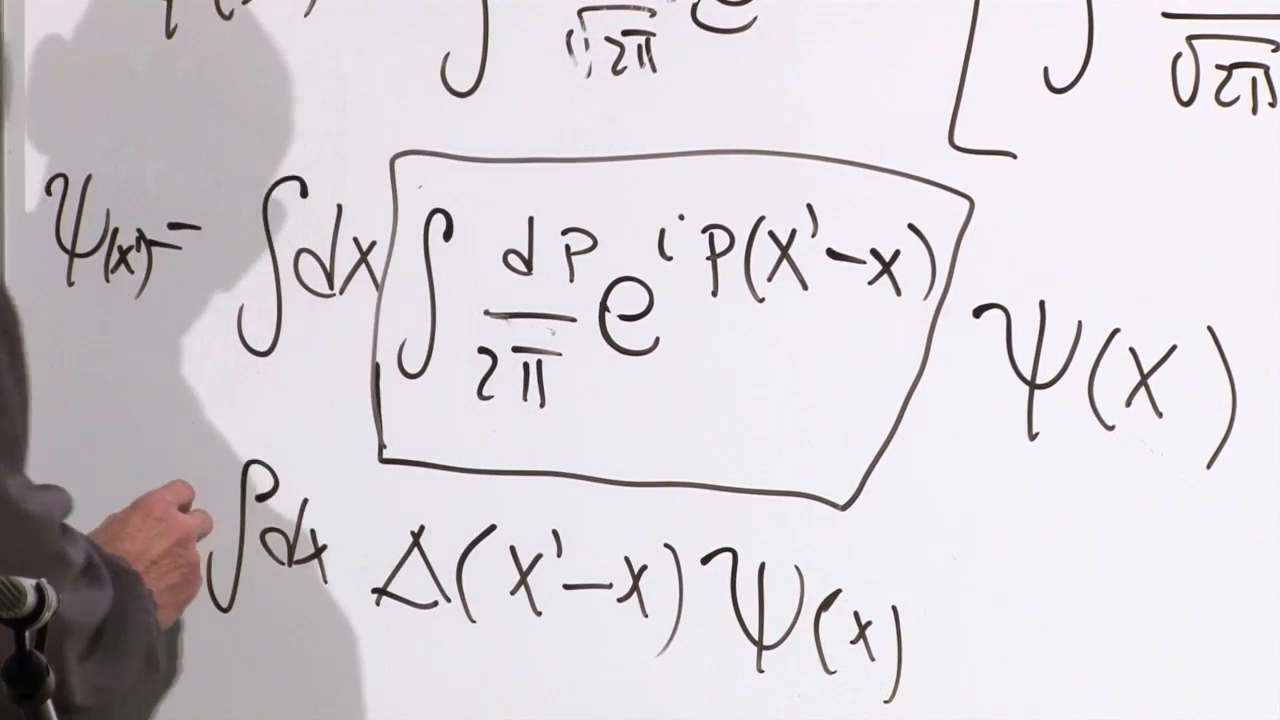
\includegraphics[width=0.88\textwidth]{lecture_09_figure_03.png}
\caption{La propriété d’échantillonnage qui caractérise la distribution de Dirac par son action sur toute fonction appropriée.}
\lectureframe{00:19:45}
\end{figure}

\begin{classroomqa}
\audiencequestion{Pourquoi peut-on sortir \(f(x')\) de l’intégrale en \(x\) ?}
\lecturerresponse{La variable d’intégration est \(x\). L’étiquette \(x'\) est fixe pendant cette intégration ; \(f(x')\) est donc constante par rapport à \(x\). L’intégrale restante de la distribution delta a une aire unité.}
\end{classroomqa}

La distribution delta n’est pas une fonction ordinaire définie point par point. En particulier, tenter de l’élever au carré produit un objet encore plus singulier que la distribution delta elle-même. Son interprétation sûre est celle d’une distribution : l’équation~\eqref{eq:l9-delta-sampling} précise son action sous une intégrale.

\subsection{Représentation de Fourier de la distribution delta}

Insérons l’équation~\eqref{eq:l9-fourier-inverse} dans l’équation~\eqref{eq:l9-fourier-forward}, en renommant \(x'\) l’argument figurant à gauche :
\begin{align}
\psi(x')
&=
\int\frac{dp}{\sqrt{2\pi}}\,
e^{ipx'}
\left[
\int\frac{dx}{\sqrt{2\pi}}\,
\psi(x)e^{-ipx}
\right] \notag\\
&=
\int dx
\left[
\int\frac{dp}{2\pi}
e^{ip(x'-x)}
\right]\psi(x).
\label{eq:l9-fourier-composition}
\end{align}
L’expression entre crochets doit reproduire \(\psi(x')\) pour toute fonction appropriée \(\psi\). En la comparant à l’action définissante de la distribution delta, on obtient
\begin{equation}
\boxed{
\int_{-\infty}^{\infty}
\frac{dp}{2\pi}\,
e^{ip(x'-x)}
=\delta(x'-x)
}.
\label{eq:l9-delta-fourier-x}
\end{equation}

\begin{figure}[htbp]
\centering
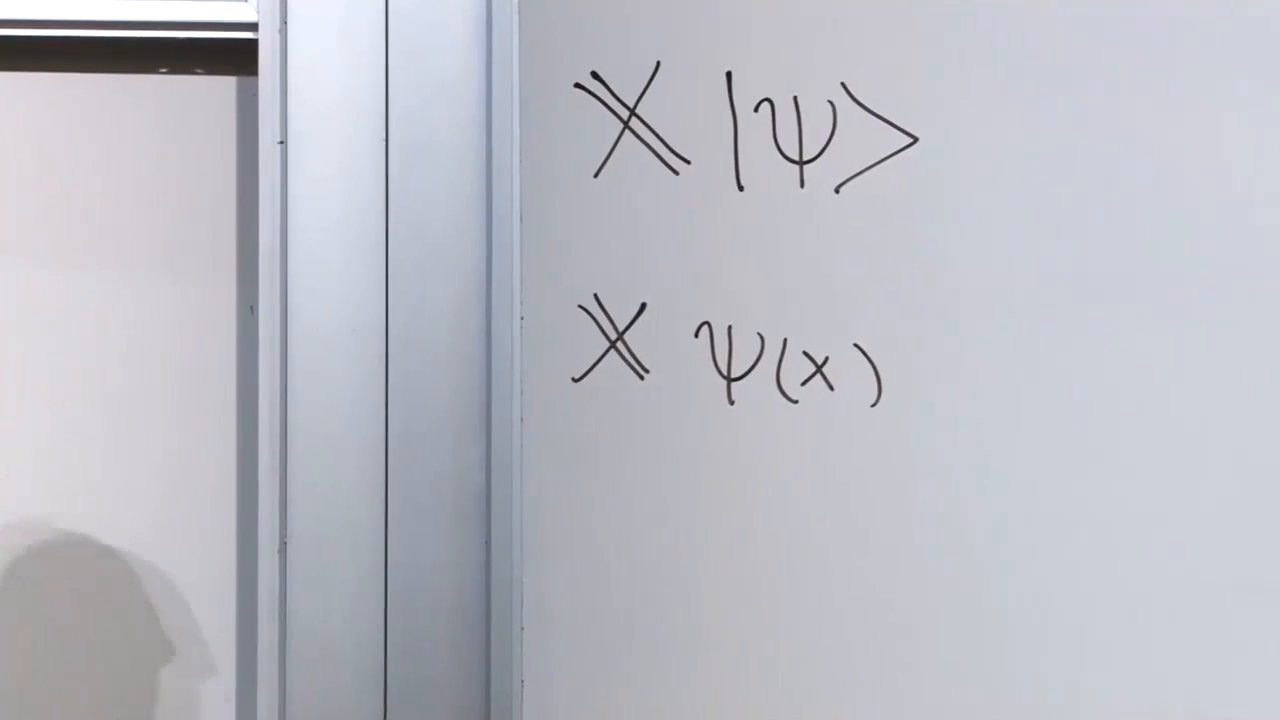
\includegraphics[width=0.88\textwidth]{lecture_09_figure_04.png}
\caption{Le noyau de Fourier est isolé dans la composition des deux transformées et identifié comme une distribution de Dirac par son action d’échantillonnage.}
\lectureframe{00:26:23}
\end{figure}

En échangeant les noms des variables réciproques, on obtient l’identité correspondante
\begin{equation}
\boxed{
\int_{-\infty}^{\infty}
\frac{dx}{2\pi}\,
e^{ix(p-p')}
=\delta(p-p')
}.
\label{eq:l9-delta-fourier-p}
\end{equation}
La distribution delta est donc une superposition continue d’ondes planes.

\begin{classroomqa}
\audiencequestion{L’exposant a été écrit une fois sous la forme \(x'-x\) et ailleurs sous la forme \(x-x'\). Le changement de signe modifie-t-il le résultat ?}
\lecturerresponse{Non. La distribution delta est paire : \(\delta(u)=\delta(-u)\). Inverser le signe de la différence laisse donc inchangée la distribution finale. L’exponentielle intermédiaire devient sa conjuguée complexe, mais le noyau intégré reste la même distribution delta.}
\end{classroomqa}

Ces manipulations passent sous silence une réserve concernant la convergence. Les intégrales oscillantes sont des distributions, et non des intégrales ordinaires absolument convergentes ; il faut donc procéder avec précaution lorsqu’on change l’ordre d’intégration. Un intervalle périodique fini fournit un régulateur commode : on commence par utiliser des modes de Fourier discrets et l’orthogonalité de Kronecker, puis on fait tendre la longueur de l’intervalle vers l’infini. Les identités continues ci-dessus sont la limite ainsi obtenue.

\section{Une particule sur une droite}

En mécanique classique, un point de l’espace des phases suffit à spécifier l’état :
\begin{equation}
(x,p).
\end{equation}
La mécanique quantique pose d’abord une autre question : quelle base orthonormale définit l’espace des états ? Pour chaque position réelle \(x\), introduisons un vecteur propre généralisé \(\ket{x}\). Un état général peut se développer ainsi :
\begin{equation}
\ket{\Psi}
=
\int_{-\infty}^{\infty}
dx\,\psi(x)\ket{x},
\qquad
\psi(x)=\braket{x}{\Psi}.
\label{eq:l9-position-expansion}
\end{equation}

\begin{figure}[htbp]
\centering
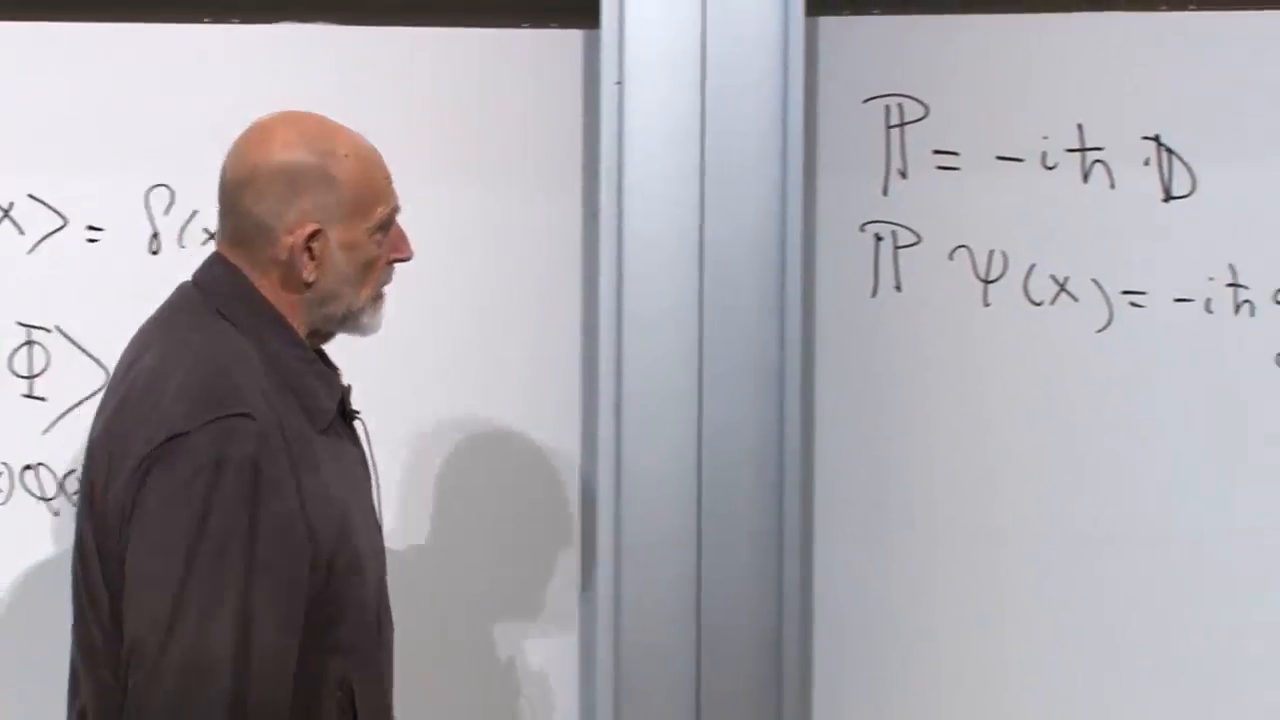
\includegraphics[width=0.88\textwidth]{lecture_09_figure_05.png}
\caption{Un état général développé dans la base continue de position, dont le coefficient s’obtient par projection sur \(\ket{x}\).}
\lectureframe{00:35:30}
\end{figure}

La règle de Born attribue la densité de probabilité
\begin{equation}
\rho(x)=|\psi(x)|^2.
\end{equation}
La probabilité dans un intervalle fini est
\begin{equation}
P(a<x<b)=\int_a^b|\psi(x)|^2\,dx,
\end{equation}
et un état physique normalisé satisfait
\begin{equation}
\int_{-\infty}^{\infty}|\psi(x)|^2\,dx=1.
\label{eq:l9-position-normalization}
\end{equation}
L’orthogonalité continue s’exprime par
\begin{equation}
\braket{x'}{x}=\delta(x-x').
\label{eq:l9-position-delta}
\end{equation}
Pour deux états quelconques, le produit scalaire devient
\begin{equation}
\braket{\Psi}{\Phi}
=
\int_{-\infty}^{\infty}
dx\,\psi^*(x)\phi(x).
\label{eq:l9-position-inner-product}
\end{equation}

\begin{figure}[htbp]
\centering
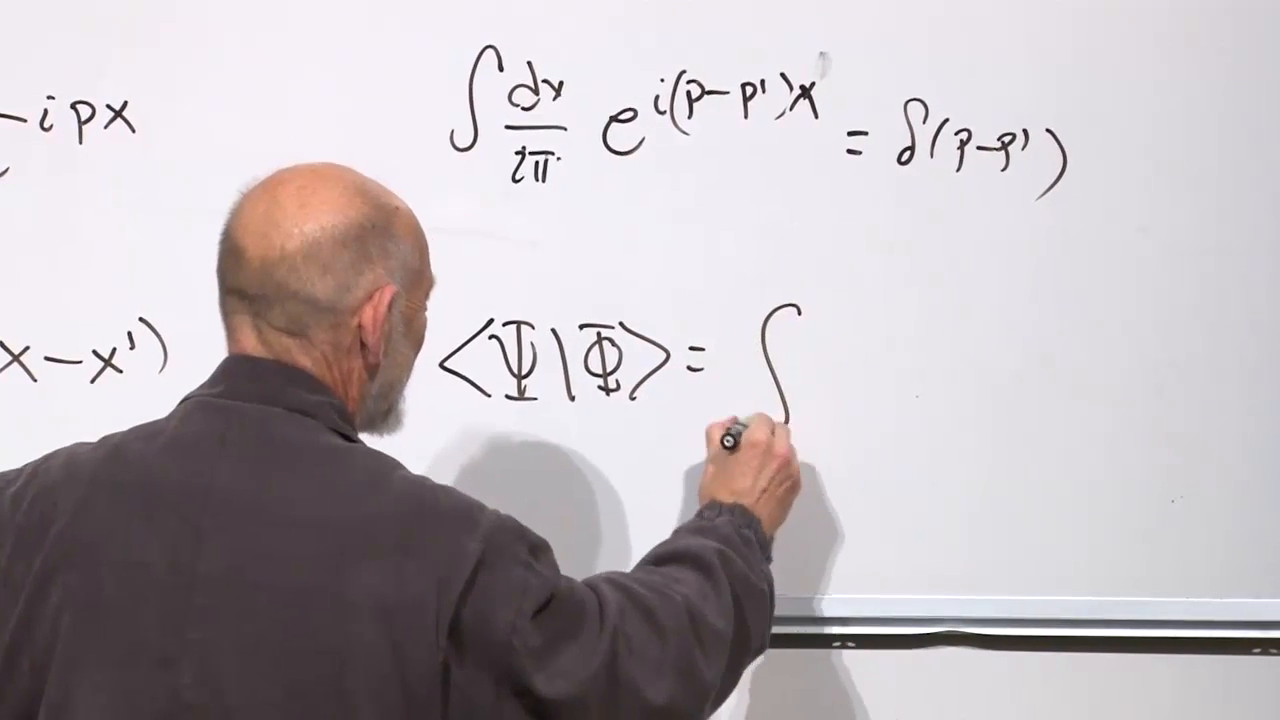
\includegraphics[width=0.88\textwidth]{lecture_09_figure_06.png}
\caption{Normalisation de la base continue et produit scalaire des fonctions d’onde écrits dans la représentation de position.}
\lectureframe{00:41:20}
\end{figure}

\begin{classroomqa}
\audiencequestion{Pourquoi la position suffit-elle à elle seule ? Ajouter la quantité de mouvement, ou presque n’importe quelle autre variable, ferait-il double emploi ?}
\lecturerresponse{Pour une particule à une dimension, la fonction complète \(\psi(x)\) spécifie l’état ; ajouter une valeur précise simultanée de \(p\) apporterait donc trop d’information. La quantité de mouvement fournit une autre base complète, plutôt qu’une étiquette supplémentaire associée à chaque \(\ket{x}\). En plusieurs dimensions, on peut combiner des informations compatibles : par exemple, \(X\) et \(P_y\) commutent et peuvent étiqueter une base commune. La restriction porte sur les paires qui ne commutent pas, et non sur le simple nombre de symboles.}
\end{classroomqa}

\begin{classroomqa}
\audiencequestion{La quantité de mouvement peut-elle également fournir une base complète, à partir de laquelle on peut développer l’état en fonction de la position ?}
\lecturerresponse{Oui. La base de quantité de mouvement est complète, et ses coefficients sont reliés aux coefficients de position par une transformée de Fourier. C’est la construction centrale de ce cours.}
\end{classroomqa}

\section{La position dans la représentation de position}

Un opérateur abstrait agit sur les vecteurs d’état. Une fois la base choisie, cette même action devient une opération concrète sur les fonctions d’onde. Dans la représentation de position, l’opérateur position \(X\) agit par multiplication :
\begin{equation}
(X\psi)(x)=x\psi(x).
\label{eq:l9-position-operator}
\end{equation}

L’état localisé en \(x_0\) est représenté par la fonction d’onde généralisée \(\delta(x-x_0)\). En appliquant \(X\), on obtient
\begin{align}
X\delta(x-x_0)
&=
x\delta(x-x_0) \notag\\
&=
x_0\delta(x-x_0),
\label{eq:l9-position-eigenfunction}
\end{align}
où l’on a utilisé l’équation~\eqref{eq:l9-delta-multiplication}. Ainsi, \(\delta(x-x_0)\) est une fonction propre de \(X\) associée à la valeur propre \(x_0\).

\begin{figure}[htbp]
\centering
\includegraphics[width=0.88\textwidth]{lecture_09_figure_07.png}
\caption{La multiplication par \(x\) transforme l’état localisé par une distribution delta en lui-même multiplié par \(x_0\), ce qui prouve qu’il s’agit d’une fonction propre de l’opérateur position.}
\lectureframe{00:45:50}
\end{figure}

Ni \(\ket{x_0}\) ni sa représentation par une distribution delta ne sont normalisés à un au sens ordinaire de l’intégrabilité au carré. Leur normalisation est celle de Dirac. Les états localisés physiques sont des paquets d’ondes de largeur finie, tandis que les états propres exacts servent de vecteurs de base généralisés.

\section{Fonctions propres de la quantité de mouvement}

Le cours précédent a établi que la dérivation est anti-hermitienne et que la multiplication par \(-i\) la rend hermitienne. En rétablissant les unités, définissons
\begin{equation}
P=-i\hbar\frac{d}{dx},
\qquad
(P\psi)(x)
=
-i\hbar\frac{d\psi}{dx}.
\label{eq:l9-momentum-operator}
\end{equation}
C’est une observable légitime sur un domaine approprié. Son identification à la quantité de mouvement physique sera vérifiée au moyen de son spectre, de sa longueur d’onde et de son rôle dans la dynamique.

Pour une valeur propre de quantité de mouvement \(p\), résolvons
\begin{equation}
P\psi_p=p\psi_p,
\end{equation}
soit
\begin{equation}
-i\hbar\frac{d\psi_p}{dx}=p\psi_p.
\end{equation}
La solution est
\begin{equation}
\psi_p(x)=A e^{ipx/\hbar}.
\label{eq:l9-momentum-eigenfunction}
\end{equation}

\begin{figure}[htbp]
\centering
\includegraphics[width=0.88\textwidth]{lecture_09_figure_08.png}
\caption{La représentation en position d’un état de quantité de mouvement déterminée est une onde plane \(e^{ipx/\hbar}\).}
\lectureframe{00:51:45}
\end{figure}

La longueur d’onde \(\lambda\) est le déplacement qui augmente la phase de \(2\pi\) :
\begin{equation}
\frac{p\lambda}{\hbar}=2\pi,
\qquad
\lambda=\frac{2\pi\hbar}{p}.
\label{eq:l9-de-broglie}
\end{equation}
Une quantité de mouvement plus grande correspond donc à une longueur d’onde plus courte.

La normalisation de Dirac fixe la constante :
\begin{equation}
\psi_p(x)
=
\frac{1}{\sqrt{2\pi\hbar}}e^{ipx/\hbar}.
\label{eq:l9-normalized-momentum-eigenfunction}
\end{equation}
En effet,
\begin{align}
\braket{p'}{p}
&=
\int_{-\infty}^{\infty}
dx\,
\psi_{p'}^*(x)\psi_p(x) \notag\\
&=
\int_{-\infty}^{\infty}
\frac{dx}{2\pi\hbar}
e^{i(p-p')x/\hbar} \notag\\
&=
\delta(p-p').
\label{eq:l9-momentum-normalization}
\end{align}
Après avoir choisi des unités telles que \(\hbar=1\), ces formules deviennent
\begin{equation}
\psi_p(x)=\frac{1}{\sqrt{2\pi}}e^{ipx},
\qquad
\int\frac{dx}{2\pi}e^{i(p-p')x}
=\delta(p-p').
\end{equation}

\begin{classroomqa}
\audiencequestion{Comment peut-on déclarer nulle l’intégrale oscillante pour \(p\neq p'\) alors qu’elle ne converge pas au sens ordinaire ?}
\lecturerresponse{Le cours adopte ici un raccourci contrôlé. Plaçons le système sur un intervalle périodique fini. Les quantités de mouvement permises forment alors un ensemble discret, les exponentielles sont orthogonales au sens ordinaire et toutes les normalisations sont finies. Ce n’est qu’après ce calcul qu’il faut faire tendre l’intervalle vers l’infini, transformant le symbole de Kronecker en distribution de Dirac.}
\end{classroomqa}

\begin{classroomqa}
\audiencequestion{Le même problème de convergence affecte-t-il la dérivation de la distribution delta par transformée de Fourier ?}
\lecturerresponse{Oui. Pour la même raison, l’échange des intégrations y était formel. La dérivation dans une boîte finie ou le langage des distributions apporte la rigueur omise. Ce raccourci est acceptable parce que le calcul régularisé possède la limite continue indiquée.}
\end{classroomqa}

\section{La représentation de quantité de mouvement}

Il ne faut pas confondre deux objets. La fonction \(\psi_p(x)\) dans l’équation~\eqref{eq:l9-normalized-momentum-eigenfunction} est la représentation en position de l’état propre particulier \(\ket{p}\). En revanche, la fonction d’onde en quantité de mouvement d’un état quelconque \(\ket{\Psi}\) est
\begin{equation}
\widetilde{\psi}(p)=\braket{p}{\Psi}.
\label{eq:l9-momentum-wavefunction}
\end{equation}
Insérons les fonctions d’onde en position de \(\bra{p}\) et de \(\ket{\Psi}\) :
\begin{align}
\widetilde{\psi}(p)
&=
\int_{-\infty}^{\infty}
dx\,
\braket{p}{x}\braket{x}{\Psi} \notag\\
&=
\int_{-\infty}^{\infty}
\frac{dx}{\sqrt{2\pi\hbar}}\,
e^{-ipx/\hbar}\psi(x).
\label{eq:l9-position-to-momentum}
\end{align}
C’est exactement la transformée de Fourier. Réciproquement,
\begin{equation}
\psi(x)
=
\int_{-\infty}^{\infty}
\frac{dp}{\sqrt{2\pi\hbar}}\,
\widetilde{\psi}(p)e^{ipx/\hbar}.
\label{eq:l9-momentum-to-position}
\end{equation}

\begin{figure}[htbp]
\centering
\includegraphics[width=0.88\textwidth]{lecture_09_figure_09.png}
\caption{La projection sur \(\ket{p}\) transforme la fonction d’onde en position en sa transformée de Fourier \(\widetilde{\psi}(p)\).}
\lectureframe{01:05:50}
\end{figure}

La densité de probabilité de mesurer la quantité de mouvement \(p\) est
\begin{equation}
\widetilde{\rho}(p)
=
|\widetilde{\psi}(p)|^2,
\qquad
\int_{-\infty}^{\infty}
|\widetilde{\psi}(p)|^2\,dp=1.
\end{equation}
Une seule fonction d’onde en position contient donc assez d’information pour prédire les mesures de position comme celles de quantité de mouvement. Pour obtenir les probabilités de quantité de mouvement, on transforme \(\psi(x)\) par Fourier et on prend le carré du module du résultat.

Dans la représentation de quantité de mouvement, les rôles s’inversent :
\begin{equation}
(P\widetilde{\psi})(p)
=
p\widetilde{\psi}(p),
\qquad
(X\widetilde{\psi})(p)
=
i\hbar\frac{d\widetilde{\psi}}{dp}.
\label{eq:l9-operators-in-p}
\end{equation}
La différence de signe par rapport à \(P=-i\hbar\,d/dx\) découle des signes opposés dans la paire de Fourier.

\begin{classroomqa}
\audiencequestion{Le temps est-il l’opérateur conjugué à l’énergie, de la même manière que la position est conjuguée à la quantité de mouvement ?}
\lecturerresponse{Le temps est généralement traité comme le paramètre externe qui étiquette l’évolution de l’état, et non comme un opérateur auto-adjoint universel sur l’espace de Hilbert du système. Une horloge physique possède bien des indications observables, et améliorer sa résolution temporelle a des conséquences sur l’énergie, mais la relation temps-énergie demande davantage de précautions que la paire position-quantité de mouvement et n’est pas développée ici.}
\end{classroomqa}

\begin{classroomqa}
\audiencequestion{Quelles autres paires conjuguées existe-t-il ?}
\lecturerresponse{L’angle et le moment cinétique correspondant en fournissent un exemple important, avec des réserves globales dues à la périodicité de l’angle. En théorie des champs, un champ et sa quantité de mouvement canonique sont conjugués. La température et la pression sont des variables thermodynamiques, et non une paire quantique canonique. Le principe général vient des variables canoniques et de leurs commutateurs, et non d’une paire quelconque de grandeurs mesurables.}
\end{classroomqa}

\begin{classroomqa}
\audiencequestion{Dans la théorie discrète, les opérateurs agissaient sur les kets et les fonctions d’onde ne faisaient que lister des coefficients. Est-ce différent dans la théorie continue ?}
\lecturerresponse{Non. Une fonction d’onde est la colonne de coordonnées d’un ket abstrait dans une base choisie. Une matrice agissant sur une colonne finie et un opérateur différentiel ou intégral agissant sur une fonction sont deux représentations concrètes d’une même opération abstraite. Le fait que l’étiquette soit continue change la notation, pas la logique.}
\end{classroomqa}

\subsection{L’incertitude comme propriété de Fourier}

Un état de quantité de mouvement déterminée est entièrement délocalisé :
\begin{equation}
|\psi_p(x)|^2=\text{constant}.
\end{equation}
Sa quantité de mouvement est bien définie, mais sa position est uniformément étalée sur toute la droite. Plus généralement, deux fonctions liées par Fourier ne peuvent pas être toutes deux concentrées dans un intervalle étroit. Concentrer \(\widetilde{\psi}(p)\) dans une petite plage de quantités de mouvement oblige \(\psi(x)\) à s’étendre sur une vaste région, tandis que localiser \(\psi(x)\) exige une large gamme de quantités de mouvement.

Le cours ne dérive pas encore l’inégalité quantitative
\begin{equation}
\Delta X\,\Delta P\geq\frac{\hbar}{2}.
\end{equation}
L’idée présentée ici est structurelle : le principe d’incertitude est déjà inscrit dans la géométrie réciproque des transformées de Fourier. C’est l’analogue continu du passage entre des bases de spin incompatibles.

\section{Le Hamiltonien engendre l’évolution temporelle}

Le Hamiltonien \(H\) est hermitien, représente l’énergie et engendre l’évolution temporelle unitaire. L’équation de Schr\"odinger dépendant du temps est
\begin{equation}
i\hbar\frac{d}{dt}\ket{\Psi(t)}
=
H\ket{\Psi(t)}.
\label{eq:l9-abstract-schrodinger}
\end{equation}
Dans la représentation de position,
\begin{equation}
i\hbar\frac{\partial\psi(x,t)}{\partial t}
=
H\psi(x,t),
\label{eq:l9-position-schrodinger}
\end{equation}
où le membre de droite désigne la représentation en position choisie du Hamiltonien agissant sur la fonction.

\subsection{Un Hamiltonien linéaire volontairement simple}

Prenons
\begin{equation}
H=cP.
\label{eq:l9-linear-hamiltonian}
\end{equation}
Ce n’est pas le Hamiltonien ordinaire d’une particule libre non relativiste. Il est choisi parce que chaque étape se voit directement.

\begin{figure}[htbp]
\centering
\includegraphics[width=0.88\textwidth]{lecture_09_figure_10.png}
\caption{L’équation de Schr\"odinger et le Hamiltonien linéaire \(H=cP\), choisis comme exemple le plus simple de l’évolution d’une particule.}
\lectureframe{01:17:45}
\end{figure}

En utilisant \(P=-i\hbar\,\partial_x\),
\begin{align}
i\hbar\frac{\partial\psi}{\partial t}
&=
c\left(-i\hbar\frac{\partial}{\partial x}\right)\psi, \notag\\
\frac{\partial\psi}{\partial t}
&=
-c\frac{\partial\psi}{\partial x},
\end{align}
soit
\begin{equation}
\frac{\partial\psi}{\partial t}
+c\frac{\partial\psi}{\partial x}=0.
\label{eq:l9-transport-equation}
\end{equation}

\begin{figure}[htbp]
\centering
\includegraphics[width=0.88\textwidth]{lecture_09_figure_11.png}
\caption{Le Hamiltonien linéaire réduit l’équation de Schr\"odinger à l’équation de transport du premier ordre.}
\lectureframe{01:20:05}
\end{figure}

La solution générale est
\begin{equation}
\psi(x,t)=f(x-ct),
\label{eq:l9-rigid-translation}
\end{equation}
pour tout profil initial normalisable \(f\). À \(t=0\), le profil est \(f(x)\). Aux temps ultérieurs, chaque caractéristique s’est décalée vers la droite de \(ct\). La fonction d’onde complexe, ses parties réelle et imaginaire, ainsi que sa densité de probabilité, conservent toutes leur forme :
\begin{equation}
|\psi(x,t)|^2=|f(x-ct)|^2.
\end{equation}
Par conséquent,
\begin{equation}
\expect{X}_t=\expect{X}_0+ct.
\end{equation}

Le symbole \(c\) a été choisi pour évoquer la vitesse de la lumière. Le modèle ressemble à une excitation chirale sans masse à une dimension : chaque composante permise se déplace dans une même direction, à une même vitesse. Ce n’est pas une théorie complète du photon. Les phonons de basse énergie à une dimension, de vitesse du son fixe, constituent une autre analogie. Comme \(E=cp\), autoriser les deux signes de \(p\) autorise aussi des énergies négatives, autre signe qu’il s’agit d’un modèle pédagogique volontairement restreint.

\begin{classroomqa}
\audiencequestion{\(H=cP\) décrirait-il une particule libre quelconque si l’on remplaçait \(c\) par la vitesse de cette particule ?}
\lecturerresponse{Non. Un coefficient fixe dans \(H=cP\) signifie que toutes les composantes de quantité de mouvement ont la même vitesse. Pour une particule non relativiste, la vitesse est \(p/m\) ; elle dépend donc de la quantité de mouvement. Écrire \(vP\) avec \(v=p/m\) n’est plus linéaire en \(P\) ; cela mène à un Hamiltonien quadratique.}
\end{classroomqa}

\begin{classroomqa}
\audiencequestion{La fonction d’onde d’un électron libre ordinaire ne devrait-elle pas simplement se translater rigidement ?}
\lecturerresponse{Seule une relation de dispersion très particulière produit une translation rigide de tout profil. Un paquet d’ondes d’électron libre ordinaire comporte de nombreuses composantes de quantité de mouvement dont les phases évoluent à des rythmes différents. Son centre se déplace, mais sa forme s’étale généralement.}
\end{classroomqa}

\subsection{Comparaison classique}

Pour le Hamiltonien classique \(H=cp\), les équations de Hamilton donnent
\begin{equation}
\dot{x}=\frac{\partial H}{\partial p}=c,
\qquad
\dot{p}=-\frac{\partial H}{\partial x}=0.
\label{eq:l9-linear-hamilton-equations}
\end{equation}

\begin{figure}[htbp]
\centering
\includegraphics[width=0.88\textwidth]{lecture_09_figure_12.png}
\caption{Équations de Hamilton pour \(H=cp\) : vitesse constante vers la droite et quantité de mouvement conservée.}
\lectureframe{01:25:20}
\end{figure}

La distribution de probabilité quantique et sa valeur moyenne obéissent au même mouvement élémentaire. Cet accord rappelle concrètement pour la première fois que l’évolution quantique construite à partir d’un Hamiltonien classique doit reproduire, en un sens approprié, les équations classiques.

\section{La particule libre non relativiste}

Pour une particule ordinaire de masse \(m\) sans force, l’énergie cinétique classique est
\begin{equation}
H=\frac{p^2}{2m}.
\end{equation}
La forme quadratique traite \(p\) et \(-p\) de manière symétrique : les particules se déplaçant vers la gauche et vers la droite ont la même énergie positive. La quantification remplace \(p\) par l’opérateur \(P\) :
\begin{equation}
H=\frac{P^2}{2m}.
\label{eq:l9-free-hamiltonian}
\end{equation}
Substituons \(P=-i\hbar\,\partial_x\) dans l’équation de Schr\"odinger :
\begin{align}
i\hbar\frac{\partial\psi}{\partial t}
&=
\frac{1}{2m}
\left(-i\hbar\frac{\partial}{\partial x}\right)^2
\psi \notag\\
&=
-\frac{\hbar^2}{2m}
\frac{\partial^2\psi}{\partial x^2}.
\label{eq:l9-free-schrodinger}
\end{align}

\begin{figure}[htbp]
\centering
\includegraphics[width=0.88\textwidth]{lecture_09_figure_13.png}
\caption{L’équation de Schr\"odinger d’une particule libre, obtenue à partir de \(H=P^2/(2m)\) et \(P=-i\hbar\,\partial_x\).}
\lectureframe{01:33:50}
\end{figure}

Une composante d’onde plane de quantité de mouvement \(p\) a pour énergie
\begin{equation}
E(p)=\frac{p^2}{2m}.
\end{equation}
Contrairement au cas linéaire \(E=cp\), la pente de cette relation de dispersion dépend de \(p\) :
\begin{equation}
v_{\mathrm{group}}
=
\frac{dE}{dp}
=
\frac{p}{m}.
\end{equation}
Les différentes composantes de quantité de mouvement d’un paquet localisé se déplacent donc à des vitesses de groupe différentes. Leurs phases relatives changent, les composantes s’écartent et le paquet s’étale. La différence décisive est que \(H=cP\) transporte rigidement toute forme, tandis que \(H=P^2/(2m)\) produit le mouvement dispersif d’une particule libre.

\section{Résultats établis}

La parenthèse mathématique n’était pas séparée de la physique. Les ondes planes et la distribution de Dirac ont fourni les outils nécessaires aux bases continues. L’opérateur position agit par multiplication, l’opérateur quantité de mouvement agit par dérivation, et les états propres de quantité de mouvement sont des ondes planes. La projection d’un état quelconque sur ces états propres donne la transformée de Fourier de sa fonction d’onde en position. La position et la quantité de mouvement sont donc deux représentations concurrentes d’un même état, et leur incertitude est la largeur réciproque familière d’une paire de Fourier.

Les mêmes outils de représentation transforment ensuite un Hamiltonien en équation différentielle. Une fonction linéaire de la quantité de mouvement produit une translation rigide ; l’énergie cinétique quadratique produit l’équation de Schr\"odinger pour une particule libre et la dispersion. Le cours est passé des fondements de la mesure à la mécanique du mouvement sans changer de langage central : états, bases, observables hermitiennes, amplitudes et évolution unitaire.
